\PassOptionsToPackage{unicode=true}{hyperref} % options for packages loaded elsewhere
\PassOptionsToPackage{hyphens}{url}
%
\documentclass[]{article}
\usepackage{lmodern}
\usepackage{amssymb,amsmath}
\usepackage{ifxetex,ifluatex}
\usepackage{fixltx2e} % provides \textsubscript
\ifnum 0\ifxetex 1\fi\ifluatex 1\fi=0 % if pdftex
  \usepackage[T1]{fontenc}
  \usepackage[utf8]{inputenc}
  \usepackage{textcomp} % provides euro and other symbols
\else % if luatex or xelatex
  \usepackage{unicode-math}
  \defaultfontfeatures{Ligatures=TeX,Scale=MatchLowercase}
\fi
% use upquote if available, for straight quotes in verbatim environments
\IfFileExists{upquote.sty}{\usepackage{upquote}}{}
% use microtype if available
\IfFileExists{microtype.sty}{%
\usepackage[]{microtype}
\UseMicrotypeSet[protrusion]{basicmath} % disable protrusion for tt fonts
}{}
\IfFileExists{parskip.sty}{%
\usepackage{parskip}
}{% else
\setlength{\parindent}{0pt}
\setlength{\parskip}{6pt plus 2pt minus 1pt}
}
\usepackage{hyperref}
\hypersetup{
            pdftitle={Regression Models: Assignment 1},
            pdfauthor={Daniel Alonso},
            pdfborder={0 0 0},
            breaklinks=true}
\urlstyle{same}  % don't use monospace font for urls
\usepackage[margin=1in]{geometry}
\usepackage{color}
\usepackage{fancyvrb}
\newcommand{\VerbBar}{|}
\newcommand{\VERB}{\Verb[commandchars=\\\{\}]}
\DefineVerbatimEnvironment{Highlighting}{Verbatim}{commandchars=\\\{\}}
% Add ',fontsize=\small' for more characters per line
\usepackage{framed}
\definecolor{shadecolor}{RGB}{248,248,248}
\newenvironment{Shaded}{\begin{snugshade}}{\end{snugshade}}
\newcommand{\AlertTok}[1]{\textcolor[rgb]{0.94,0.16,0.16}{#1}}
\newcommand{\AnnotationTok}[1]{\textcolor[rgb]{0.56,0.35,0.01}{\textbf{\textit{#1}}}}
\newcommand{\AttributeTok}[1]{\textcolor[rgb]{0.77,0.63,0.00}{#1}}
\newcommand{\BaseNTok}[1]{\textcolor[rgb]{0.00,0.00,0.81}{#1}}
\newcommand{\BuiltInTok}[1]{#1}
\newcommand{\CharTok}[1]{\textcolor[rgb]{0.31,0.60,0.02}{#1}}
\newcommand{\CommentTok}[1]{\textcolor[rgb]{0.56,0.35,0.01}{\textit{#1}}}
\newcommand{\CommentVarTok}[1]{\textcolor[rgb]{0.56,0.35,0.01}{\textbf{\textit{#1}}}}
\newcommand{\ConstantTok}[1]{\textcolor[rgb]{0.00,0.00,0.00}{#1}}
\newcommand{\ControlFlowTok}[1]{\textcolor[rgb]{0.13,0.29,0.53}{\textbf{#1}}}
\newcommand{\DataTypeTok}[1]{\textcolor[rgb]{0.13,0.29,0.53}{#1}}
\newcommand{\DecValTok}[1]{\textcolor[rgb]{0.00,0.00,0.81}{#1}}
\newcommand{\DocumentationTok}[1]{\textcolor[rgb]{0.56,0.35,0.01}{\textbf{\textit{#1}}}}
\newcommand{\ErrorTok}[1]{\textcolor[rgb]{0.64,0.00,0.00}{\textbf{#1}}}
\newcommand{\ExtensionTok}[1]{#1}
\newcommand{\FloatTok}[1]{\textcolor[rgb]{0.00,0.00,0.81}{#1}}
\newcommand{\FunctionTok}[1]{\textcolor[rgb]{0.00,0.00,0.00}{#1}}
\newcommand{\ImportTok}[1]{#1}
\newcommand{\InformationTok}[1]{\textcolor[rgb]{0.56,0.35,0.01}{\textbf{\textit{#1}}}}
\newcommand{\KeywordTok}[1]{\textcolor[rgb]{0.13,0.29,0.53}{\textbf{#1}}}
\newcommand{\NormalTok}[1]{#1}
\newcommand{\OperatorTok}[1]{\textcolor[rgb]{0.81,0.36,0.00}{\textbf{#1}}}
\newcommand{\OtherTok}[1]{\textcolor[rgb]{0.56,0.35,0.01}{#1}}
\newcommand{\PreprocessorTok}[1]{\textcolor[rgb]{0.56,0.35,0.01}{\textit{#1}}}
\newcommand{\RegionMarkerTok}[1]{#1}
\newcommand{\SpecialCharTok}[1]{\textcolor[rgb]{0.00,0.00,0.00}{#1}}
\newcommand{\SpecialStringTok}[1]{\textcolor[rgb]{0.31,0.60,0.02}{#1}}
\newcommand{\StringTok}[1]{\textcolor[rgb]{0.31,0.60,0.02}{#1}}
\newcommand{\VariableTok}[1]{\textcolor[rgb]{0.00,0.00,0.00}{#1}}
\newcommand{\VerbatimStringTok}[1]{\textcolor[rgb]{0.31,0.60,0.02}{#1}}
\newcommand{\WarningTok}[1]{\textcolor[rgb]{0.56,0.35,0.01}{\textbf{\textit{#1}}}}
\usepackage{graphicx,grffile}
\makeatletter
\def\maxwidth{\ifdim\Gin@nat@width>\linewidth\linewidth\else\Gin@nat@width\fi}
\def\maxheight{\ifdim\Gin@nat@height>\textheight\textheight\else\Gin@nat@height\fi}
\makeatother
% Scale images if necessary, so that they will not overflow the page
% margins by default, and it is still possible to overwrite the defaults
% using explicit options in \includegraphics[width, height, ...]{}
\setkeys{Gin}{width=\maxwidth,height=\maxheight,keepaspectratio}
\setlength{\emergencystretch}{3em}  % prevent overfull lines
\providecommand{\tightlist}{%
  \setlength{\itemsep}{0pt}\setlength{\parskip}{0pt}}
\setcounter{secnumdepth}{0}
% Redefines (sub)paragraphs to behave more like sections
\ifx\paragraph\undefined\else
\let\oldparagraph\paragraph
\renewcommand{\paragraph}[1]{\oldparagraph{#1}\mbox{}}
\fi
\ifx\subparagraph\undefined\else
\let\oldsubparagraph\subparagraph
\renewcommand{\subparagraph}[1]{\oldsubparagraph{#1}\mbox{}}
\fi

% set default figure placement to htbp
\makeatletter
\def\fps@figure{htbp}
\makeatother


\title{Regression Models: Assignment 1}
\author{Daniel Alonso}
\date{November 24th, 2020}

\begin{document}
\maketitle

\hypertarget{installing-libraries-used}{%
\subsection{Installing libraries used}\label{installing-libraries-used}}

\begin{Shaded}
\begin{Highlighting}[]
\NormalTok{packages =}\StringTok{ }\KeywordTok{c}\NormalTok{(}\StringTok{"dplyr"}\NormalTok{,}\StringTok{"MuMIn"}\NormalTok{,}\StringTok{"MASS"}\NormalTok{,}\StringTok{"leaps"}\NormalTok{,}\StringTok{"glmnet"}\NormalTok{,}\StringTok{"car"}\NormalTok{)}
\ControlFlowTok{for}\NormalTok{ (package }\ControlFlowTok{in}\NormalTok{ packages) \{}
    \KeywordTok{install.packages}\NormalTok{(package)}
\NormalTok{\}}
\end{Highlighting}
\end{Shaded}

\hypertarget{importing-libraries}{%
\subsection{Importing libraries}\label{importing-libraries}}

\begin{Shaded}
\begin{Highlighting}[]
\KeywordTok{library}\NormalTok{(dplyr)}
\KeywordTok{library}\NormalTok{(MuMIn)}
\KeywordTok{library}\NormalTok{(MASS)}
\KeywordTok{library}\NormalTok{(leaps)}
\KeywordTok{library}\NormalTok{(glmnet)}
\KeywordTok{library}\NormalTok{(car)}
\end{Highlighting}
\end{Shaded}

\newpage

\hypertarget{exercise-1}{%
\section{Exercise 1}\label{exercise-1}}

\hypertarget{simulation}{%
\subsection{Simulation}\label{simulation}}

\begin{Shaded}
\begin{Highlighting}[]
\CommentTok{# terms}
\NormalTok{s =}\StringTok{ }\KeywordTok{list}\NormalTok{()}
\NormalTok{X =}\StringTok{ }\KeywordTok{list}\NormalTok{()}

\CommentTok{# betas estimation}
\NormalTok{beta_est =}\StringTok{ }\KeywordTok{list}\NormalTok{()}
\NormalTok{beta1hat =}\StringTok{ }\KeywordTok{c}\NormalTok{()}
\NormalTok{beta2hat =}\StringTok{ }\KeywordTok{c}\NormalTok{()}

\CommentTok{# variables}
\NormalTok{phi =}\StringTok{ }\DecValTok{50}
\NormalTok{beta1 =}\StringTok{ }\DecValTok{3}
\NormalTok{beta2 =}\StringTok{ }\DecValTok{3}
\NormalTok{x1 =}\StringTok{ }\KeywordTok{matrix}\NormalTok{(}\KeywordTok{rep}\NormalTok{(}\DecValTok{1}\NormalTok{,}\DecValTok{100}\NormalTok{),}\DataTypeTok{nrow=}\DecValTok{100}\NormalTok{,}\DataTypeTok{byrow=}\NormalTok{T)}

\CommentTok{# simulation}
\NormalTok{simulation <-}\StringTok{ }\ControlFlowTok{function}\NormalTok{(mean,sd,phi,beta1,beta2,iters,size) \{}
    \ControlFlowTok{for}\NormalTok{ (j }\ControlFlowTok{in} \DecValTok{1}\OperatorTok{:}\NormalTok{iters) \{}
\NormalTok{        loop_s =}\StringTok{ }\KeywordTok{matrix}\NormalTok{(}\KeywordTok{rep}\NormalTok{(}\DecValTok{0}\NormalTok{,size),}\DataTypeTok{nrow=}\NormalTok{size,}\DataTypeTok{byrow=}\NormalTok{T)}
\NormalTok{        loop_x2 =}\StringTok{ }\KeywordTok{matrix}\NormalTok{(}\KeywordTok{rep}\NormalTok{(}\DecValTok{0}\NormalTok{,size),}\DataTypeTok{nrow=}\NormalTok{size,}\DataTypeTok{byrow=}\NormalTok{T)}
        \ControlFlowTok{for}\NormalTok{ (i }\ControlFlowTok{in} \DecValTok{1}\OperatorTok{:}\NormalTok{size) \{}
\NormalTok{            e =}\StringTok{ }\KeywordTok{rnorm}\NormalTok{(}\DecValTok{1}\NormalTok{, }\DataTypeTok{mean=}\NormalTok{mean, }\DataTypeTok{sd=}\NormalTok{sd)}
\NormalTok{            loop_x2[i] =}\StringTok{ }\KeywordTok{cos}\NormalTok{(i}\OperatorTok{/}\DecValTok{10} \OperatorTok{+}\StringTok{ }\NormalTok{phi)}
\NormalTok{            loop_s[i] =}\StringTok{ }\NormalTok{beta1 }\OperatorTok{+}\StringTok{ }\NormalTok{beta2}\OperatorTok{*}\NormalTok{loop_x2[i] }\OperatorTok{+}\StringTok{ }\NormalTok{e}
\NormalTok{        \}}
\NormalTok{        X[[j]] =}\StringTok{ }\KeywordTok{cbind}\NormalTok{(x1,loop_x2)}
\NormalTok{        s[[j]] =}\StringTok{ }\NormalTok{loop_s}
\NormalTok{        beta_est[[j]] =}\StringTok{ }\KeywordTok{ginv}\NormalTok{(}\KeywordTok{t}\NormalTok{(X[[j]])}\OperatorTok\NormalTok{X[[j]])}\OperatorTok\KeywordTok{t}\NormalTok{(X[[j]])}\OperatorTok\NormalTok{loop_s}
\NormalTok{        beta1hat =}\StringTok{ }\KeywordTok{c}\NormalTok{(beta1hat, beta_est[[j]][}\DecValTok{1}\NormalTok{])}
\NormalTok{        beta2hat =}\StringTok{ }\KeywordTok{c}\NormalTok{(beta2hat, beta_est[[j]][}\DecValTok{2}\NormalTok{])}
\NormalTok{    \}}
    \CommentTok{# plotting beta1hat and beta2hat}
    \KeywordTok{par}\NormalTok{(}\DataTypeTok{mfrow=}\KeywordTok{c}\NormalTok{(}\DecValTok{2}\NormalTok{,}\DecValTok{1}\NormalTok{))}
    \KeywordTok{hist}\NormalTok{(beta1hat)}
    \KeywordTok{hist}\NormalTok{(beta2hat)}
    \KeywordTok{return}\NormalTok{(}\KeywordTok{c}\NormalTok{(}\KeywordTok{mean}\NormalTok{(beta1hat),}\KeywordTok{mean}\NormalTok{(beta2hat)))}
\NormalTok{\}}
\end{Highlighting}
\end{Shaded}

\newpage

\begin{Shaded}
\begin{Highlighting}[]
\NormalTok{means <-}\StringTok{ }\KeywordTok{simulation}\NormalTok{(}\DataTypeTok{mean=}\DecValTok{0}\NormalTok{, }\DataTypeTok{sd=}\DecValTok{1}\NormalTok{, }\DataTypeTok{phi=}\NormalTok{phi, }\DataTypeTok{beta1=}\NormalTok{beta1, }\DataTypeTok{beta2=}\NormalTok{beta2, }\DataTypeTok{iters=}\DecValTok{1000}\NormalTok{, }\DataTypeTok{size=}\DecValTok{100}\NormalTok{)}
\end{Highlighting}
\end{Shaded}

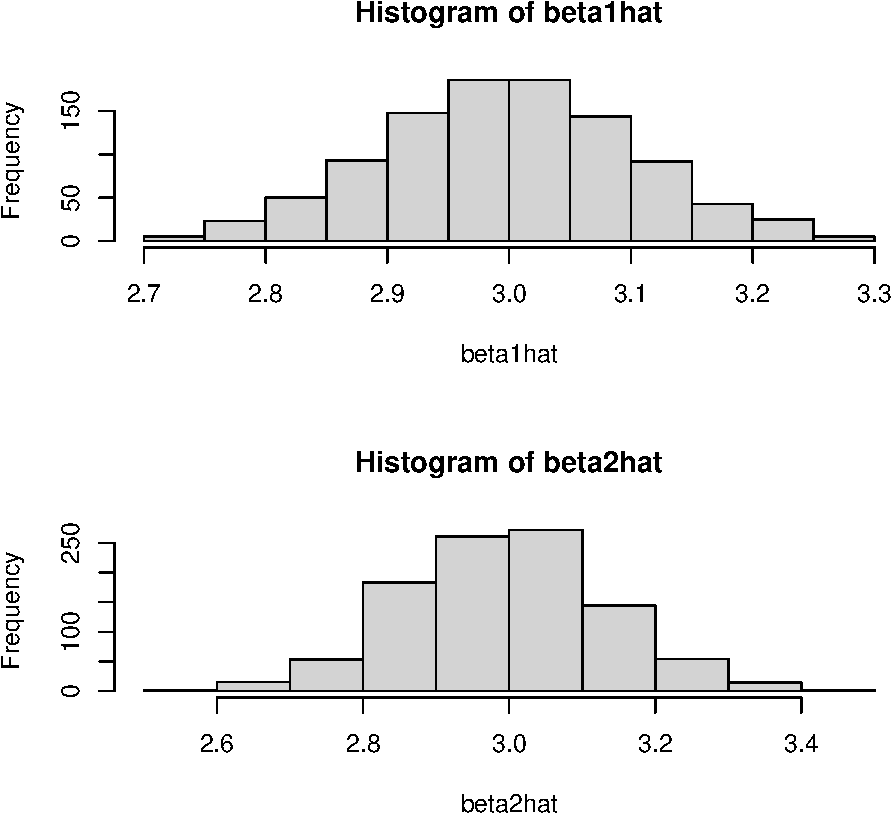
\includegraphics{./figures/unnamed-chunk-4-1.pdf}

We know that the estimate is unbiased if its expected value of our
estimators is equal to the real value of our estimators (in this case
\(E[ \hat{\beta_{1}}]) = \beta_{1}\) and
\(E[ \hat{\beta_{2}}]) = \beta_{2}\) as the sample size
\(n \rightarrow \inf\).

We can test for this with our 1000 simulation sample:

\begin{Shaded}
\begin{Highlighting}[]
\KeywordTok{print}\NormalTok{(means)}
\CommentTok{#> [1] 2.998648 2.995063}
\end{Highlighting}
\end{Shaded}

Calculating a relative error for each one of these values:

\begin{Shaded}
\begin{Highlighting}[]
\NormalTok{betas =}\StringTok{ }\KeywordTok{c}\NormalTok{(beta1,beta2)}
\ControlFlowTok{for}\NormalTok{ (i }\ControlFlowTok{in} \DecValTok{1}\OperatorTok{:}\KeywordTok{length}\NormalTok{(means)) \{}
    \KeywordTok{print}\NormalTok{(}\KeywordTok{paste}\NormalTok{(}\StringTok{"beta "}\NormalTok{,i, }\StringTok{" hat has a relative error of: "}\NormalTok{, }\KeywordTok{abs}\NormalTok{(means[i]}\OperatorTok{-}\NormalTok{betas[i])}\OperatorTok{/}\NormalTok{betas[i]))}
\NormalTok{\}   }
\CommentTok{#> [1] "beta  1  hat has a relative error of:  0.000450824739430071"}
\CommentTok{#> [1] "beta  2  hat has a relative error of:  0.00164582858190151"}
\end{Highlighting}
\end{Shaded}

Which are \textless{}1\% incorrect versus the real betas, therefore,
these estimators are unbiased.

\newpage

If we increase the value of sigma by \textasciitilde{}10x the original
value (\(\sigma = 1\)):

\begin{Shaded}
\begin{Highlighting}[]
\NormalTok{means <-}\StringTok{ }\KeywordTok{simulation}\NormalTok{(}\DataTypeTok{mean=}\DecValTok{0}\NormalTok{, }\DataTypeTok{sd=}\DecValTok{10}\NormalTok{, }\DataTypeTok{phi=}\NormalTok{phi, }\DataTypeTok{beta1=}\NormalTok{beta1, }\DataTypeTok{beta2=}\NormalTok{beta2, }\DataTypeTok{iters=}\DecValTok{1000}\NormalTok{, }\DataTypeTok{size=}\DecValTok{100}\NormalTok{)}
\end{Highlighting}
\end{Shaded}

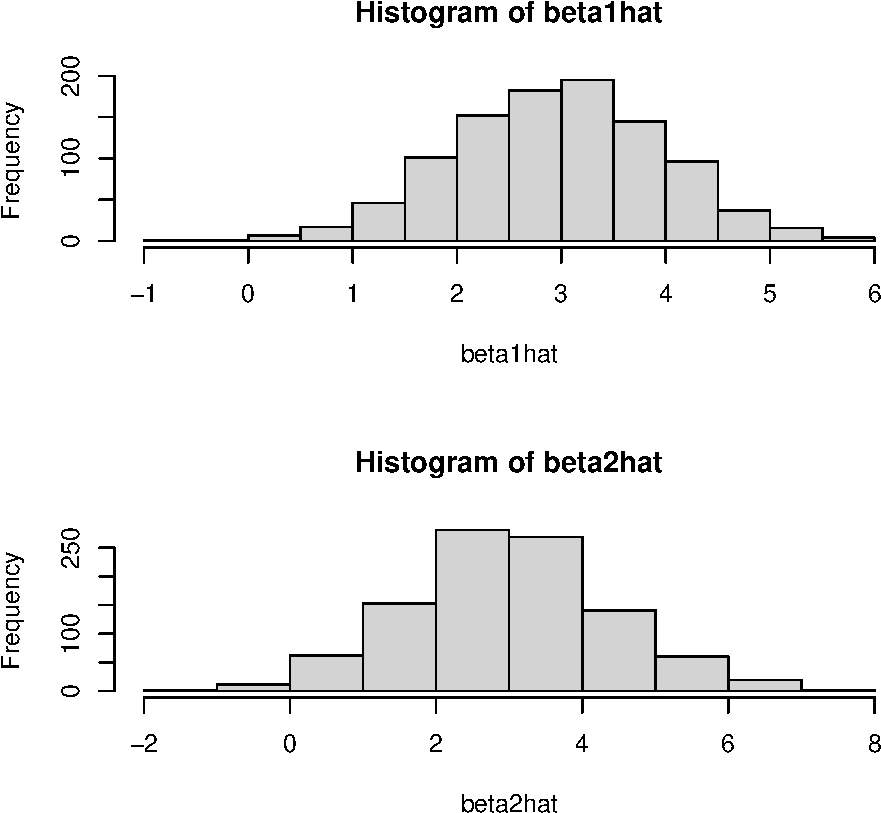
\includegraphics{./figures/unnamed-chunk-7-1.pdf}

\begin{Shaded}
\begin{Highlighting}[]
\KeywordTok{print}\NormalTok{(means)}
\CommentTok{#> [1] 3.048041 3.016336}
\end{Highlighting}
\end{Shaded}

\begin{Shaded}
\begin{Highlighting}[]
\NormalTok{betas =}\StringTok{ }\KeywordTok{c}\NormalTok{(beta1,beta2)}
\ControlFlowTok{for}\NormalTok{ (i }\ControlFlowTok{in} \DecValTok{1}\OperatorTok{:}\KeywordTok{length}\NormalTok{(means)) \{}
    \KeywordTok{print}\NormalTok{(}\KeywordTok{paste}\NormalTok{(}\StringTok{"beta "}\NormalTok{,i, }\StringTok{" hat has a relative error of: "}\NormalTok{, }\KeywordTok{abs}\NormalTok{(means[i]}\OperatorTok{-}\NormalTok{betas[i])}\OperatorTok{/}\NormalTok{betas[i]))}
\NormalTok{\}}
\CommentTok{#> [1] "beta  1  hat has a relative error of:  0.0160135157751419"}
\CommentTok{#> [1] "beta  2  hat has a relative error of:  0.00544517964421646"}
\end{Highlighting}
\end{Shaded}

We can see that our relative error increases, therefore our estimation
would either require a significantly larger amount of iterations to
reach a the same estimation accuracy. So then we could say that our
residuals being a lot more disperse can measurably affect the accuracy
of our prediction.

\newpage

If we increase the value of sigma by \textasciitilde{}1000x the original
value (\(\sigma = 1\)):

\begin{Shaded}
\begin{Highlighting}[]
\NormalTok{means <-}\StringTok{ }\KeywordTok{simulation}\NormalTok{(}\DataTypeTok{mean=}\DecValTok{0}\NormalTok{, }\DataTypeTok{sd=}\DecValTok{1000}\NormalTok{, }\DataTypeTok{phi=}\NormalTok{phi, }\DataTypeTok{beta1=}\NormalTok{beta1, }\DataTypeTok{beta2=}\NormalTok{beta2, }\DataTypeTok{iters=}\DecValTok{1000}\NormalTok{, }\DataTypeTok{size=}\DecValTok{100}\NormalTok{)}
\end{Highlighting}
\end{Shaded}

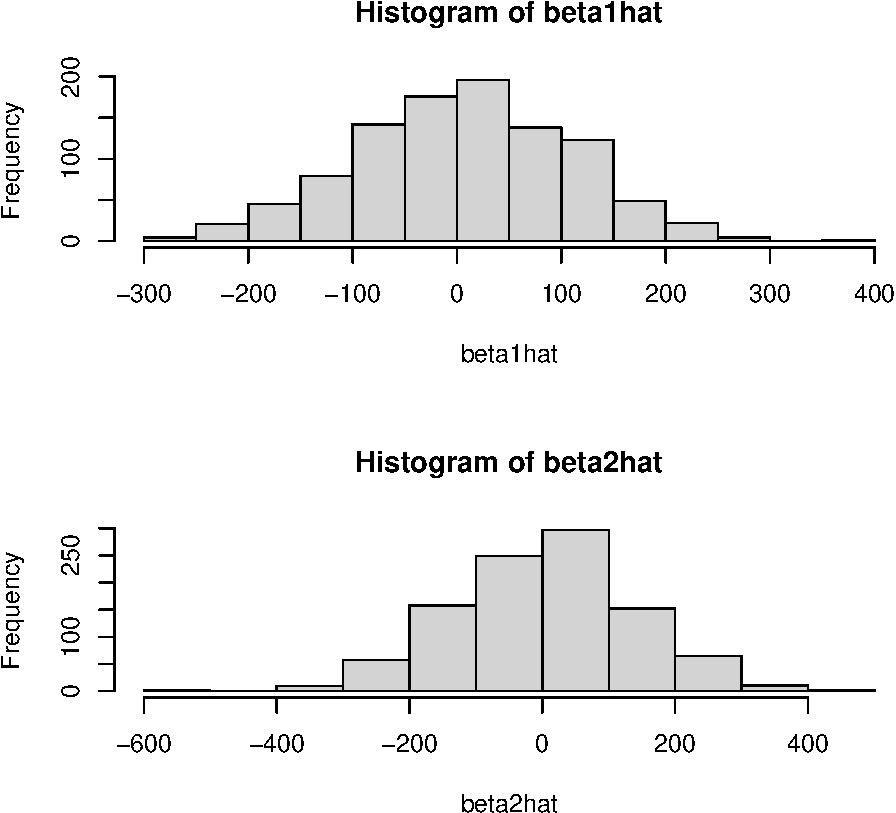
\includegraphics{./figures/unnamed-chunk-10-1.pdf}

\begin{Shaded}
\begin{Highlighting}[]
\KeywordTok{print}\NormalTok{(means)}
\CommentTok{#> [1]  1.773244 11.106923}
\end{Highlighting}
\end{Shaded}

\begin{Shaded}
\begin{Highlighting}[]
\NormalTok{betas =}\StringTok{ }\KeywordTok{c}\NormalTok{(beta1,beta2)}
\ControlFlowTok{for}\NormalTok{ (i }\ControlFlowTok{in} \DecValTok{1}\OperatorTok{:}\KeywordTok{length}\NormalTok{(means)) \{}
    \KeywordTok{print}\NormalTok{(}\KeywordTok{paste}\NormalTok{(}\StringTok{"beta "}\NormalTok{,i, }\StringTok{" hat has a relative error of: "}\NormalTok{, }\KeywordTok{abs}\NormalTok{(means[i]}\OperatorTok{-}\NormalTok{betas[i])}\OperatorTok{/}\NormalTok{betas[i]))}
\NormalTok{\}}
\CommentTok{#> [1] "beta  1  hat has a relative error of:  0.408918539601745"}
\CommentTok{#> [1] "beta  2  hat has a relative error of:  2.70230766346048"}
\end{Highlighting}
\end{Shaded}

In an attempt to show a waaaaay worse scenario, here we can see our
relative error is not only large but, having tried running this a few
times, the relative error can reach massive amounts, being, at times,
even way higher than 100\% wrong.

\newpage

\hypertarget{exercise-2}{%
\section{Exercise 2}\label{exercise-2}}

\hypertarget{importing-the-data}{%
\subsection{Importing the data}\label{importing-the-data}}

\begin{Shaded}
\begin{Highlighting}[]
\NormalTok{d <-}\StringTok{ }\KeywordTok{data.frame}\NormalTok{(}\KeywordTok{read.table}\NormalTok{(}\StringTok{'../data/index.txt'}\NormalTok{, }\DataTypeTok{header=}\OtherTok{TRUE}\NormalTok{))}
\end{Highlighting}
\end{Shaded}

\begin{Shaded}
\begin{Highlighting}[]
\NormalTok{X =}\StringTok{ }\NormalTok{d}\OperatorTok{$}\NormalTok{PovPct}
\NormalTok{Y =}\StringTok{ }\NormalTok{d}\OperatorTok{$}\NormalTok{Brth15to17}
\NormalTok{beta1 =}\StringTok{ }\KeywordTok{cov}\NormalTok{(X, Y)}\OperatorTok{/}\KeywordTok{var}\NormalTok{(X)}
\NormalTok{beta0 =}\StringTok{ }\KeywordTok{mean}\NormalTok{(Y) }\OperatorTok{-}\StringTok{ }\NormalTok{beta1}\OperatorTok{*}\KeywordTok{mean}\NormalTok{(X)}
\end{Highlighting}
\end{Shaded}

\begin{Shaded}
\begin{Highlighting}[]
\NormalTok{beta1}
\CommentTok{#> [1] 1.373345}
\NormalTok{beta0}
\CommentTok{#> [1] 4.267293}
\end{Highlighting}
\end{Shaded}

\hypertarget{exercise-3}{%
\section{Exercise 3}\label{exercise-3}}

First we have the log-likelihood function for \(\beta\) and
\(\sigma^{2}\)

\(l(\sigma^{2} | X) = \sum_{i=1}^n log(\frac{1}{\sqrt{2 \pi \sigma^{2}}} - \frac{(Y_{i} - (\beta_{0} + \beta_{1} x_{ik} + \dots + \beta_{k} x_{ik}))^{2}}{2 \sigma^{2}})\)

\(\propto - \frac{n}{2} log(\sigma^{2}) - \frac{(Y - X \beta) \prime (Y - X \beta)}{2 \sigma^{2}}\)

Differentiating the second expression:

\(\frac{\partial l}{\partial \sigma} ( - \frac{n}{2} log(\sigma^{2}) - \frac{(Y - X \beta) \prime (Y - X \beta)}{2 \sigma^{2}}) = 0\)

We get:

\(- \frac{n}{2} (\frac{1}{ \sigma^{2}} ) (2 \sigma) - (Y - X \beta) \prime (Y - X \beta) * (-2)(2 \sigma^{-3}) = 0\)

We reduce the expression further:

\(- \frac{n}{\sigma} + \frac{(Y - X \beta) \prime (Y - X \beta)}{\sigma^{3}} = 0\)

We multiply both sides by \(\sigma^{3}\) and we get:

\(- n \sigma^{2} + (Y - X \beta) \prime (Y - X \beta) = 0\)

And solving for \(\sigma^{2}\) we get:

\(\hat{\sigma^{2}} = \frac{(Y - X \beta) \prime (Y - X \beta)}{n}\)

Which is our maximum likelihood estimator for \(\sigma^2\)

\newpage

\hypertarget{exercise-4}{%
\section{Exercise 4}\label{exercise-4}}

1- \(\sum_{i=1}^n \hat{\epsilon_i}\)

\newpage

\hypertarget{exercise-5}{%
\section{Exercise 5}\label{exercise-5}}

\begin{Shaded}
\begin{Highlighting}[]
\NormalTok{bodyfat <-}\StringTok{ }\KeywordTok{data.frame}\NormalTok{(}\KeywordTok{read.table}\NormalTok{(}\StringTok{'../data/bodyfat.txt'}\NormalTok{, }\DataTypeTok{header=}\OtherTok{TRUE}\NormalTok{))}
\NormalTok{modall <-}\StringTok{ }\KeywordTok{lm}\NormalTok{(hwfat }\OperatorTok{~}\NormalTok{., }\DataTypeTok{data =}\NormalTok{ bodyfat)}
\KeywordTok{summary}\NormalTok{(modall)}
\CommentTok{#> }
\CommentTok{#> Call:}
\CommentTok{#> lm(formula = hwfat ~ ., data = bodyfat)}
\CommentTok{#> }
\CommentTok{#> Residuals:}
\CommentTok{#>    Min     1Q Median     3Q    Max }
\CommentTok{#> -6.162 -1.858 -0.464  2.502  8.177 }
\CommentTok{#> }
\CommentTok{#> Coefficients:}
\CommentTok{#>             Estimate Std. Error t value Pr(>|t|)    }
\CommentTok{#> (Intercept) 13.29370    9.63027   1.380   0.1718    }
\CommentTok{#> age         -0.32893    0.32158  -1.023   0.3098    }
\CommentTok{#> ht          -0.06731    0.16051  -0.419   0.6762    }
\CommentTok{#> wt          -0.01365    0.02591  -0.527   0.5999    }
\CommentTok{#> abs          0.37142    0.08837   4.203 7.55e-05 ***}
\CommentTok{#> triceps      0.38743    0.13761   2.815   0.0063 ** }
\CommentTok{#> subscap      0.11405    0.14193   0.804   0.4243    }
\CommentTok{#> ---}
\CommentTok{#> Signif. codes:  0 '***' 0.001 '**' 0.01 '*' 0.05 '.' 0.1 ' ' 1}
\CommentTok{#> }
\CommentTok{#> Residual standard error: 3.028 on 71 degrees of freedom}
\CommentTok{#> Multiple R-squared:  0.8918, Adjusted R-squared:  0.8827 }
\CommentTok{#> F-statistic: 97.54 on 6 and 71 DF,  p-value: < 2.2e-16}
\end{Highlighting}
\end{Shaded}

The sum of residuals is zero:

\begin{Shaded}
\begin{Highlighting}[]
\NormalTok{residuals <-}\StringTok{ }\KeywordTok{sum}\NormalTok{(}\KeywordTok{resid}\NormalTok{(modall))}
\end{Highlighting}
\end{Shaded}

The sum of the observed data is equal to the sum of the fitted values

\begin{Shaded}
\begin{Highlighting}[]
\NormalTok{Y_hat <-}\StringTok{ }\KeywordTok{predict}\NormalTok{(modall, bodyfat[}\DecValTok{1}\OperatorTok{:}\KeywordTok{length}\NormalTok{(}\KeywordTok{names}\NormalTok{(bodyfat))}\OperatorTok{-}\DecValTok{1}\NormalTok{])}
\KeywordTok{sum}\NormalTok{(bodyfat}\OperatorTok{$}\NormalTok{hwfat) }\OperatorTok{-}\StringTok{ }\KeywordTok{sum}\NormalTok{(Y_hat)}
\CommentTok{#> [1] 4.547474e-13}
\end{Highlighting}
\end{Shaded}

The residuals are orthogonal to the predictors

\begin{Shaded}
\begin{Highlighting}[]
\KeywordTok{sum}\NormalTok{(residuals}\OperatorTok{*}\NormalTok{bodyfat[}\DecValTok{1}\OperatorTok{:}\KeywordTok{length}\NormalTok{(}\KeywordTok{names}\NormalTok{(bodyfat))}\OperatorTok{-}\DecValTok{1}\NormalTok{])}
\CommentTok{#> [1] -3.077268e-10}
\end{Highlighting}
\end{Shaded}

The residuals are orthogonal to the fitted values

\begin{Shaded}
\begin{Highlighting}[]
\KeywordTok{sum}\NormalTok{(residuals}\OperatorTok{*}\NormalTok{Y_hat)}
\CommentTok{#> [1] -1.568657e-11}
\end{Highlighting}
\end{Shaded}

\newpage

\hypertarget{exercise-6}{%
\section{Exercise 6}\label{exercise-6}}

We use regsubsets to find the best model combinations by adjusted
\(R^{2}\)

\begin{Shaded}
\begin{Highlighting}[]
\KeywordTok{options}\NormalTok{(}\DataTypeTok{na.action =} \StringTok{"na.fail"}\NormalTok{)}
\NormalTok{modall <-}\StringTok{ }\KeywordTok{lm}\NormalTok{(hwfat }\OperatorTok{~}\NormalTok{., }\DataTypeTok{data =}\NormalTok{ bodyfat)}
\NormalTok{combs <-}\StringTok{ }\NormalTok{leaps}\OperatorTok{::}\KeywordTok{regsubsets}\NormalTok{(bodyfat[,}\DecValTok{1}\OperatorTok{:}\DecValTok{6}\NormalTok{],bodyfat[,}\DecValTok{7}\NormalTok{])}
\KeywordTok{summary}\NormalTok{(combs)}
\CommentTok{#> Subset selection object}
\CommentTok{#> 6 Variables  (and intercept)}
\CommentTok{#>         Forced in Forced out}
\CommentTok{#> age         FALSE      FALSE}
\CommentTok{#> ht          FALSE      FALSE}
\CommentTok{#> wt          FALSE      FALSE}
\CommentTok{#> abs         FALSE      FALSE}
\CommentTok{#> triceps     FALSE      FALSE}
\CommentTok{#> subscap     FALSE      FALSE}
\CommentTok{#> 1 subsets of each size up to 6}
\CommentTok{#> Selection Algorithm: exhaustive}
\CommentTok{#>          age ht  wt  abs triceps subscap}
\CommentTok{#> 1  ( 1 ) " " " " " " "*" " "     " "    }
\CommentTok{#> 2  ( 1 ) " " " " " " "*" "*"     " "    }
\CommentTok{#> 3  ( 1 ) "*" " " " " "*" "*"     " "    }
\CommentTok{#> 4  ( 1 ) "*" "*" " " "*" "*"     " "    }
\CommentTok{#> 5  ( 1 ) "*" " " "*" "*" "*"     "*"    }
\CommentTok{#> 6  ( 1 ) "*" "*" "*" "*" "*"     "*"}
\end{Highlighting}
\end{Shaded}

And their corresponding \$R\^{}\{2\} values:

\begin{Shaded}
\begin{Highlighting}[]
\KeywordTok{summary}\NormalTok{(combs)}\OperatorTok{$}\NormalTok{adjr2}
\CommentTok{#> [1] 0.8409068 0.8801014 0.8849817 0.8846381 0.8840129 0.8826699}
\end{Highlighting}
\end{Shaded}

We can see the best model is the one with the following \(R^{2}\)

\begin{Shaded}
\begin{Highlighting}[]
\KeywordTok{max}\NormalTok{(}\KeywordTok{summary}\NormalTok{(combs}\OperatorTok{$}\NormalTok{adjr2))}
\CommentTok{#> [1] "NULL"}
\end{Highlighting}
\end{Shaded}

Which corresponds to the model which uses the variables \textbf{age},
\textbf{ht}, \textbf{abs} and \textbf{triceps}.

We can also do this same calculation using the function dredge (albeit
less efficiently):

\begin{Shaded}
\begin{Highlighting}[]
\NormalTok{combs <-}\StringTok{ }\KeywordTok{dredge}\NormalTok{(modall, }\DataTypeTok{extra =} \StringTok{"R^2"}\NormalTok{)}
\KeywordTok{print}\NormalTok{(}\StringTok{"best model"}\NormalTok{)}
\CommentTok{#> [1] "best model"}
\NormalTok{combs[combs}\OperatorTok{$}\StringTok{"R^2"} \OperatorTok{==}\StringTok{ }\KeywordTok{max}\NormalTok{(combs}\OperatorTok{$}\StringTok{"R^2"}\NormalTok{)]}
\CommentTok{#> Global model call: lm(formula = hwfat ~ ., data = bodyfat)}
\CommentTok{#> ---}
\CommentTok{#> Model selection table }
\CommentTok{#>    (Intrc)    abs     age       ht  sbscp  trcps       wt    R^2 df  logLik}
\CommentTok{#> 64   13.29 0.3714 -0.3289 -0.06731 0.1141 0.3874 -0.01365 0.8918  8 -193.43}
\CommentTok{#>     AICc delta weight}
\CommentTok{#> 64 404.9  5.58      1}
\CommentTok{#> Models ranked by AICc(x)}
\end{Highlighting}
\end{Shaded}

\newpage

\hypertarget{exercise-7}{%
\section{Exercise 7}\label{exercise-7}}

We know that:

\(SST = \sum_{i=1}^{n} (y_{i}-\bar{y})^{2}\\ = \sum_{i=1}^{n} (y_{i} - \hat{y_{i}} + \hat{y_{i}} - \bar{y})^{2}\\ = \sum_{i=1}^{n} (y_{i} - \hat{y_{i}})^{2} + 2 \sum_{i=1}^{n} (y_{i} - \hat{y_{i}}) (\hat{y_{i}} - \bar{y}) + \sum_{i=1}^{n} (\hat{y_{i}} - \bar{y})^{2}\\ = SSE + SSR + 2 \sum_{i=1}^{n} (y_{i}-\hat{y_{i}})(\hat{y_{i}}-\bar{y})\)

No we must prove that:

\(2 \sum_{i=1}^{n} (y_{i}-\hat{y_{i}})(\hat{y_{i}}-\bar{y}) = 0\)

So then we have:

\(\sum_{i=1}^{n} (y_{i}-\hat{y_{i}})(\hat{y_{i}}-\bar{y}) = \sum_{i=1}^{n} (y_{i} - \hat{y_{i}}) \hat{y_{i}} - \sum_{i=1}^{n} (y_{i} - \hat{y_{i}}) \bar{y} = 0\)

Because we know that:

\(\sum_{i=1}^{n} (y_{i} - \hat{y_{i}}) \hat{y_{i}} = 0\)

Given that the residuals must be orthogonal to the fitted values.

And:

\(\sum_{i=1}^{n} (y_{i} - \hat{y_{i}}) \bar{y} = 0\)

Because the sum of the observed data is equal to the sum of the fitted
values:

\(\sum_{i=1}^{n} y_{i} = \sum_{i=1}^{n} \hat{y_{i}}\)

\newpage

\hypertarget{exercise-8}{%
\section{Exercise 8}\label{exercise-8}}

We define a list with all the models excluding, in each one, a single
variable.

\begin{Shaded}
\begin{Highlighting}[]
\NormalTok{models <-}\StringTok{ }\KeywordTok{list}\NormalTok{()}
\NormalTok{vars <-}\StringTok{ }\KeywordTok{c}\NormalTok{(}\StringTok{"age"}\NormalTok{,}\StringTok{"ht"}\NormalTok{,}\StringTok{"wt"}\NormalTok{,}\StringTok{"abs"}\NormalTok{,}\StringTok{"triceps"}\NormalTok{,}\StringTok{"subscap"}\NormalTok{)}
\NormalTok{models[[}\DecValTok{1}\NormalTok{]] <-}\StringTok{ }\KeywordTok{update}\NormalTok{(modall,.}\OperatorTok{~}\NormalTok{.}\OperatorTok{-}\NormalTok{age)}
\NormalTok{models[[}\DecValTok{2}\NormalTok{]] <-}\StringTok{ }\KeywordTok{update}\NormalTok{(modall,.}\OperatorTok{~}\NormalTok{.}\OperatorTok{-}\NormalTok{ht)}
\NormalTok{models[[}\DecValTok{3}\NormalTok{]] <-}\StringTok{ }\KeywordTok{update}\NormalTok{(modall,.}\OperatorTok{~}\NormalTok{.}\OperatorTok{-}\NormalTok{wt)}
\NormalTok{models[[}\DecValTok{4}\NormalTok{]] <-}\StringTok{ }\KeywordTok{update}\NormalTok{(modall,.}\OperatorTok{~}\NormalTok{.}\OperatorTok{-}\NormalTok{abs)}
\NormalTok{models[[}\DecValTok{5}\NormalTok{]] <-}\StringTok{ }\KeywordTok{update}\NormalTok{(modall,.}\OperatorTok{~}\NormalTok{.}\OperatorTok{-}\NormalTok{triceps)}
\NormalTok{models[[}\DecValTok{6}\NormalTok{]] <-}\StringTok{ }\KeywordTok{update}\NormalTok{(modall,.}\OperatorTok{~}\NormalTok{.}\OperatorTok{-}\NormalTok{subscap)}
\end{Highlighting}
\end{Shaded}

We run ANOVA with both the models without each variable and the main
model including all the other variables.

We can see the pvalues for the ANOVA where each specific variable was
excluded:

\begin{Shaded}
\begin{Highlighting}[]
\NormalTok{anovas <-}\StringTok{ }\KeywordTok{list}\NormalTok{()}
\NormalTok{pvalues <-}\StringTok{ }\KeywordTok{c}\NormalTok{()}
\NormalTok{amount_of_vars <-}\StringTok{ }\KeywordTok{length}\NormalTok{(}\KeywordTok{names}\NormalTok{(bodyfat))}\OperatorTok{-}\DecValTok{1}
\ControlFlowTok{for}\NormalTok{ (i }\ControlFlowTok{in} \DecValTok{1}\OperatorTok{:}\NormalTok{amount_of_vars) \{}
\NormalTok{    anovas[[i]] <-}\StringTok{ }\KeywordTok{anova}\NormalTok{(models[[i]],modall)}
\NormalTok{    pvalues <-}\StringTok{ }\KeywordTok{c}\NormalTok{(pvalues, }\KeywordTok{sum}\NormalTok{(anovas[[i]][}\DecValTok{2}\NormalTok{,}\StringTok{"Pr(>F)"}\NormalTok{]))}
\NormalTok{\}}
\ControlFlowTok{for}\NormalTok{ (i }\ControlFlowTok{in} \DecValTok{1}\OperatorTok{:}\KeywordTok{length}\NormalTok{(vars)) \{}
    \KeywordTok{print}\NormalTok{(}\KeywordTok{paste}\NormalTok{(}\StringTok{"excluding: "}\NormalTok{, vars[i], }\StringTok{": "}\NormalTok{, pvalues[i] , }\DataTypeTok{sep=}\StringTok{""}\NormalTok{))}
\NormalTok{\}}
\CommentTok{#> [1] "excluding: age: 0.30983932449522"}
\CommentTok{#> [1] "excluding: ht: 0.67622546378066"}
\CommentTok{#> [1] "excluding: wt: 0.599878887504826"}
\CommentTok{#> [1] "excluding: abs: 7.54898491342447e-05"}
\CommentTok{#> [1] "excluding: triceps: 0.00630111253287972"}
\CommentTok{#> [1] "excluding: subscap: 0.424314507846979"}
\end{Highlighting}
\end{Shaded}

Then we compare with summary:

\begin{Shaded}
\begin{Highlighting}[]
\KeywordTok{summary}\NormalTok{(modall)[}\DecValTok{4}\NormalTok{]}
\CommentTok{#> $coefficients}
\CommentTok{#>                Estimate Std. Error    t value     Pr(>|t|)}
\CommentTok{#> (Intercept) 13.29369860 9.63026704  1.3804081 1.717917e-01}
\CommentTok{#> age         -0.32893403 0.32157778 -1.0228755 3.098393e-01}
\CommentTok{#> ht          -0.06730905 0.16050751 -0.4193514 6.762255e-01}
\CommentTok{#> wt          -0.01365183 0.02590783 -0.5269385 5.998789e-01}
\CommentTok{#> abs          0.37141976 0.08836595  4.2032001 7.548985e-05}
\CommentTok{#> triceps      0.38742647 0.13761017  2.8153912 6.301113e-03}
\CommentTok{#> subscap      0.11405213 0.14192779  0.8035927 4.243145e-01}
\end{Highlighting}
\end{Shaded}

And we can see we get the same pvalues in the summary. Therefore viewing
the summary can be a much faster version of performing such testing.

as a result we get that the least meaningful variable (the variable that
explains the lowest variance of the model) is the variable ht (height)
followed by the variable wt (weight).

\newpage

\hypertarget{exercise-9}{%
\section{Exercise 9}\label{exercise-9}}

Given that
\(E[\hat{Y} | X_{h}] = \hat{Y_{h}} \sim N(X_{h} \beta, \sigma^{2} X_{h} (X^{\prime} X) X_{h}^{\prime})\)

\(\Rightarrow \hat{y_{h}} \pm t_{n - (k+1), \frac{\alpha}{2}} * \hat{\sigma} \sqrt{h_{ii}}\)

where \(h_{ii}\) is the diagonal of our \(H\) matrix.

is our expression for the \((1-\alpha)\%\) confidence interval for
\(\hat{Y_{h}}\) when \(\sigma^{2}\) is unknown.

\hypertarget{exercise-10}{%
\section{Exercise 10}\label{exercise-10}}

\begin{Shaded}
\begin{Highlighting}[]
\NormalTok{minmax_scaler <-}\StringTok{ }\ControlFlowTok{function}\NormalTok{(x) \{}
    \KeywordTok{return}\NormalTok{((x}\OperatorTok{-}\KeywordTok{min}\NormalTok{(x))}\OperatorTok{/}\NormalTok{(}\KeywordTok{max}\NormalTok{(x)}\OperatorTok{-}\KeywordTok{min}\NormalTok{(x)))}
\NormalTok{\}}
\end{Highlighting}
\end{Shaded}

\begin{Shaded}
\begin{Highlighting}[]
\NormalTok{transform <-}\StringTok{ }\KeywordTok{data.frame}\NormalTok{(}\KeywordTok{read.table}\NormalTok{(}\StringTok{'../data/Transform_V2.txt'}\NormalTok{, }\DataTypeTok{header=}\OtherTok{TRUE}\NormalTok{))}
\NormalTok{trm1 <-}\StringTok{ }\KeywordTok{lm}\NormalTok{(y }\OperatorTok{~}\StringTok{ }\KeywordTok{sqrt}\NormalTok{(x2}\OperatorTok{+}\DecValTok{1}\NormalTok{), }\DataTypeTok{data=}\NormalTok{transform)}
\NormalTok{trm2 <-}\StringTok{ }\KeywordTok{lm}\NormalTok{(y }\OperatorTok{~}\StringTok{ }\KeywordTok{I}\NormalTok{(x3}\OperatorTok{^}\NormalTok{(}\DecValTok{2}\NormalTok{)), }\DataTypeTok{data=}\NormalTok{transform)}
\KeywordTok{par}\NormalTok{(}\DataTypeTok{mfrow=}\KeywordTok{c}\NormalTok{(}\DecValTok{2}\NormalTok{,}\DecValTok{2}\NormalTok{))}
\KeywordTok{plot}\NormalTok{(trm1)}
\end{Highlighting}
\end{Shaded}

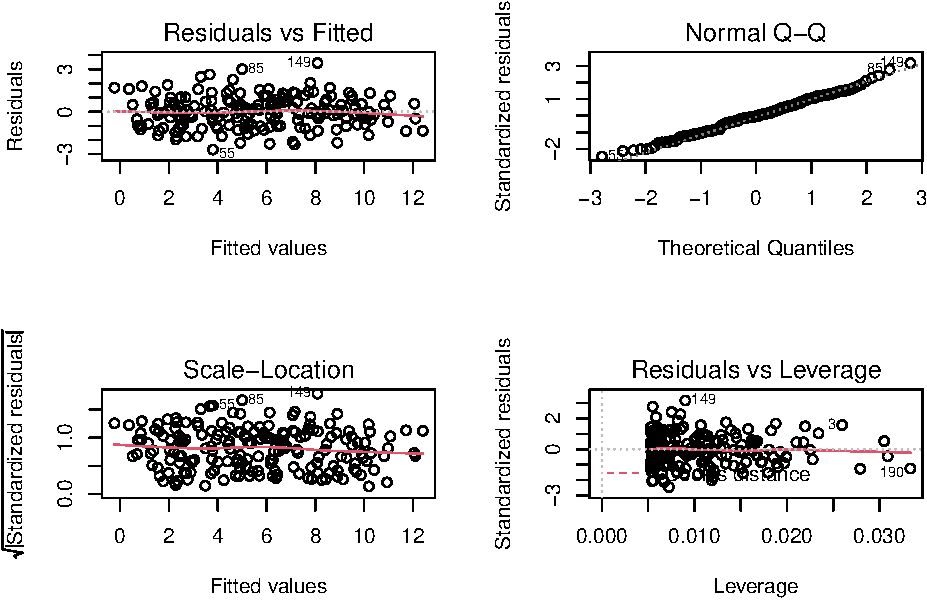
\includegraphics{./figures/unnamed-chunk-29-1.pdf}

We can see that the square root transformation is appropriate for the
\(X_{2}\) variable

\newpage

\begin{Shaded}
\begin{Highlighting}[]
\KeywordTok{par}\NormalTok{(}\DataTypeTok{mfrow=}\KeywordTok{c}\NormalTok{(}\DecValTok{2}\NormalTok{,}\DecValTok{2}\NormalTok{))}
\KeywordTok{plot}\NormalTok{(trm2)}
\end{Highlighting}
\end{Shaded}

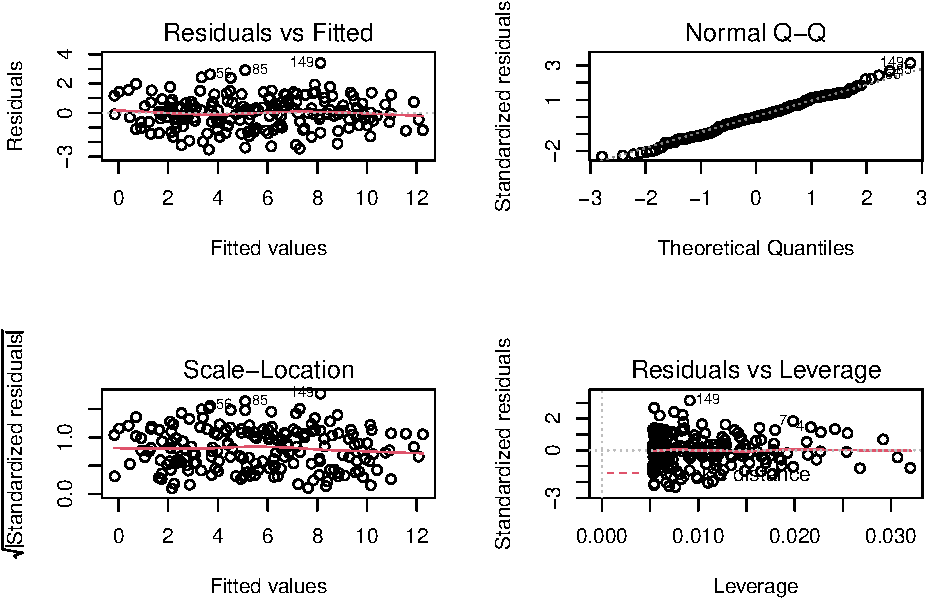
\includegraphics{./figures/unnamed-chunk-30-1.pdf}

We can see that the \(X^{2}\) transformation is appropriate for the
\(X_{3}\) variable

\newpage

\hypertarget{exercise-11}{%
\section{Exercise 11}\label{exercise-11}}

\begin{Shaded}
\begin{Highlighting}[]
\NormalTok{bxcx_transf <-}\StringTok{ }\ControlFlowTok{function}\NormalTok{(x, lambda) \{}
    \ControlFlowTok{if}\NormalTok{ (lambda }\OperatorTok{==}\StringTok{ }\DecValTok{0}\NormalTok{) \{}
        \KeywordTok{return}\NormalTok{(}\KeywordTok{log}\NormalTok{(x))}
\NormalTok{    \} }\ControlFlowTok{else}\NormalTok{ \{}
        \KeywordTok{return}\NormalTok{((x}\OperatorTok{^}\NormalTok{(lambda)}\OperatorTok{-}\DecValTok{1}\NormalTok{)}\OperatorTok{/}\NormalTok{lambda)}
\NormalTok{    \}}
\NormalTok{\}}
\end{Highlighting}
\end{Shaded}

\begin{Shaded}
\begin{Highlighting}[]
\NormalTok{transform2 <-}\StringTok{ }\KeywordTok{data.frame}\NormalTok{(}\KeywordTok{read.table}\NormalTok{(}\StringTok{'../data/Transform2_V2.txt'}\NormalTok{, }\DataTypeTok{header=}\OtherTok{TRUE}\NormalTok{))}
\NormalTok{trm1 <-}\StringTok{ }\KeywordTok{lm}\NormalTok{(y2 }\OperatorTok{~}\StringTok{ }\NormalTok{x1, }\DataTypeTok{data=}\NormalTok{transform2)}
\NormalTok{trm2 <-}\StringTok{ }\KeywordTok{lm}\NormalTok{(y2 }\OperatorTok{~}\StringTok{ }\NormalTok{x2, }\DataTypeTok{data=}\NormalTok{transform2)}
\KeywordTok{par}\NormalTok{(}\DataTypeTok{mfrow=}\KeywordTok{c}\NormalTok{(}\DecValTok{2}\NormalTok{,}\DecValTok{4}\NormalTok{))}
\KeywordTok{plot}\NormalTok{(trm1)}
\KeywordTok{plot}\NormalTok{(trm2)}
\end{Highlighting}
\end{Shaded}

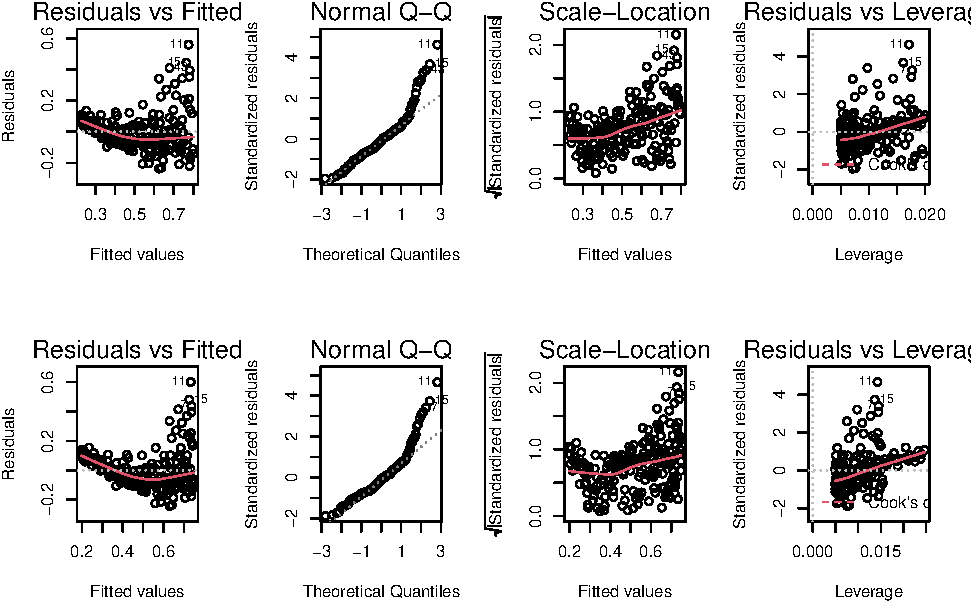
\includegraphics{./figures/unnamed-chunk-32-1.pdf}

Neither variable has constant variance, therefore we apply a boxcox
transformation to both \(X_{2}\) and \(X_{3}\).

\newpage

\begin{Shaded}
\begin{Highlighting}[]
\KeywordTok{boxcox}\NormalTok{(trm2)}
\end{Highlighting}
\end{Shaded}

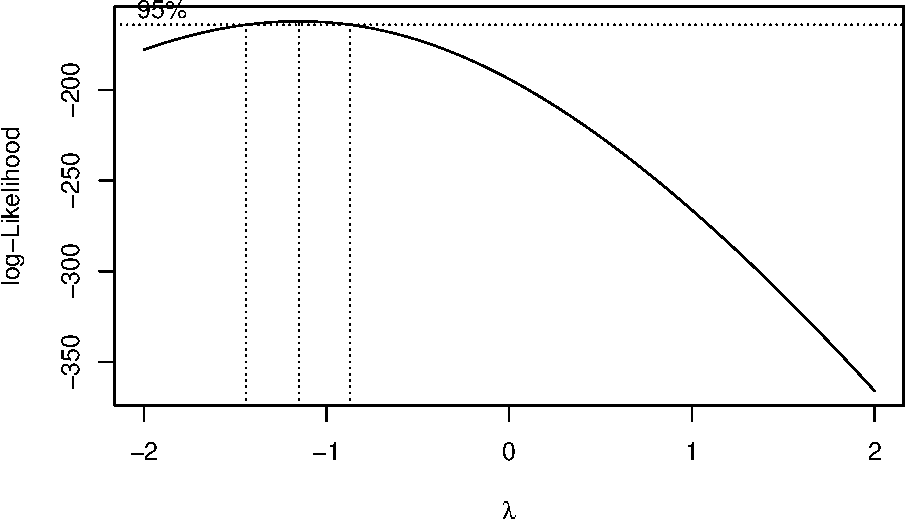
\includegraphics{./figures/unnamed-chunk-33-1.pdf}

\begin{Shaded}
\begin{Highlighting}[]
\KeywordTok{boxcox}\NormalTok{(trm1)}
\end{Highlighting}
\end{Shaded}

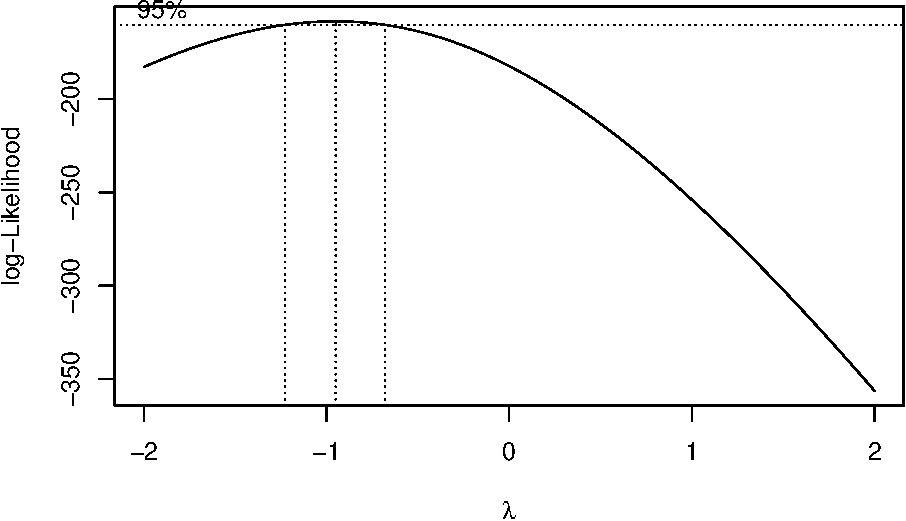
\includegraphics{./figures/unnamed-chunk-34-1.pdf}

\newpage

As \(-1\) is in the confidence interval for both models, we will apply a
boxcox transformation using \(\lambda = -1\).

\begin{Shaded}
\begin{Highlighting}[]
\NormalTok{transform2 <-}\StringTok{ }\KeywordTok{data.frame}\NormalTok{(}\KeywordTok{read.table}\NormalTok{(}\StringTok{'../data/Transform2_V2.txt'}\NormalTok{, }\DataTypeTok{header=}\OtherTok{TRUE}\NormalTok{))}
\NormalTok{trm1 <-}\StringTok{ }\KeywordTok{lm}\NormalTok{(}\KeywordTok{bxcx_transf}\NormalTok{(y2,}\OperatorTok{-}\DecValTok{1}\NormalTok{) }\OperatorTok{~}\StringTok{ }\NormalTok{x1, }\DataTypeTok{data=}\NormalTok{transform2)}
\NormalTok{trm2 <-}\StringTok{ }\KeywordTok{lm}\NormalTok{(}\KeywordTok{bxcx_transf}\NormalTok{(y2,}\OperatorTok{-}\DecValTok{1}\NormalTok{) }\OperatorTok{~}\StringTok{ }\NormalTok{x2, }\DataTypeTok{data=}\NormalTok{transform2)}
\KeywordTok{par}\NormalTok{(}\DataTypeTok{mfrow=}\KeywordTok{c}\NormalTok{(}\DecValTok{2}\NormalTok{,}\DecValTok{4}\NormalTok{))}
\KeywordTok{plot}\NormalTok{(trm1)}
\KeywordTok{plot}\NormalTok{(trm2)}
\end{Highlighting}
\end{Shaded}

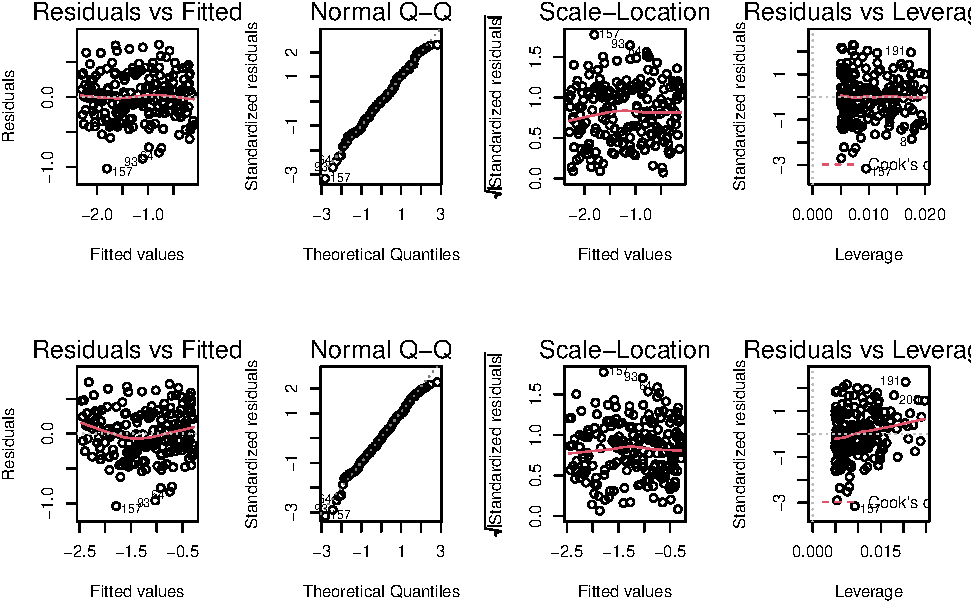
\includegraphics{./figures/unnamed-chunk-35-1.pdf}

Here we see the situation has improved significantly and we now have
constant variance.

\newpage

\hypertarget{exercise-12}{%
\section{Exercise 12}\label{exercise-12}}

\newpage

\hypertarget{exercise-13}{%
\section{Exercise 13}\label{exercise-13}}

Using R's function to calculate VIF for our model:

\begin{Shaded}
\begin{Highlighting}[]
\KeywordTok{vif}\NormalTok{(modall)}
\CommentTok{#>       age        ht        wt       abs   triceps   subscap }
\CommentTok{#>  1.553994  2.582940 10.194274 10.799321 10.951090 14.114459}
\end{Highlighting}
\end{Shaded}

We can see that the VIF score for \textbf{triceps}, \textbf{abs},
\textbf{wt} and \textbf{subscap} are all above 10 and therefore very
high.

Programming my own VIF function:

The approach here is to set up a linear model using the variable who's
VIF score we want to calculate in each loop using its predictors as its
predictors (basically passing through the function the section of our
dataframe that corresponds to predictor variables).

Essentially doing the following:

\(X_{1} = k_{1} + k_{2} X_{2} + k_{3} X_{3} + \dots + k_{n} X_{n}\)

Where each \(k_{i}\) is a constant, and each \(X_{i}\) is a predictor.

Then we calculate the VIF score for each one of them using the
coefficient of determination of the fitted values of the model and the
real values of the predictor that we set as dependent variable in the
model corresponding to that loop and adding these elements to a list.

\begin{Shaded}
\begin{Highlighting}[]
\NormalTok{vif_mc <-}\StringTok{ }\ControlFlowTok{function}\NormalTok{(X) \{}
\NormalTok{    result <-}\StringTok{ }\KeywordTok{c}\NormalTok{()}
    \ControlFlowTok{for}\NormalTok{ (i }\ControlFlowTok{in} \DecValTok{1}\OperatorTok{:}\NormalTok{(}\KeywordTok{length}\NormalTok{(}\KeywordTok{names}\NormalTok{(X)))) \{}
\NormalTok{        variables <-}\StringTok{ }\KeywordTok{names}\NormalTok{(X)}
\NormalTok{        preds <-}\StringTok{ }\DecValTok{1}\OperatorTok{:}\KeywordTok{length}\NormalTok{(}\KeywordTok{names}\NormalTok{(X))}
\NormalTok{        preds <-}\StringTok{ }\NormalTok{preds[preds }\OperatorTok{!=}\StringTok{ }\NormalTok{i]}
\NormalTok{        other_vars <-}\StringTok{ ""}
        \ControlFlowTok{for}\NormalTok{ (j }\ControlFlowTok{in} \DecValTok{1}\OperatorTok{:}\NormalTok{(}\KeywordTok{length}\NormalTok{(}\KeywordTok{names}\NormalTok{(X))}\OperatorTok{-}\DecValTok{1}\NormalTok{)) \{}
\NormalTok{            ov =}\StringTok{ }\NormalTok{variables[variables }\OperatorTok{!=}\StringTok{ }\NormalTok{variables[i]]}
            \ControlFlowTok{if}\NormalTok{ (j }\OperatorTok{>}\StringTok{ }\DecValTok{1}\NormalTok{) \{}
\NormalTok{                other_vars =}\StringTok{ }\KeywordTok{paste}\NormalTok{(other_vars, }\StringTok{"+"}\NormalTok{ ,ov[j])}
\NormalTok{            \} }\ControlFlowTok{else}\NormalTok{ \{}
\NormalTok{                other_vars =}\StringTok{ }\NormalTok{ov[j]}
\NormalTok{            \}}
            
\NormalTok{        \}}
\NormalTok{        model <-}\StringTok{ }\KeywordTok{lm}\NormalTok{(}\KeywordTok{paste}\NormalTok{(variables[i], }\StringTok{"~"}\NormalTok{, other_vars), }\DataTypeTok{data=}\NormalTok{X)}
\NormalTok{        result <-}\StringTok{ }\KeywordTok{c}\NormalTok{(result, }\DecValTok{1}\OperatorTok{/}\NormalTok{(}\DecValTok{1}\OperatorTok{-}\NormalTok{((}\KeywordTok{cor}\NormalTok{(X[i],}\KeywordTok{fitted}\NormalTok{(model)))}\OperatorTok{^}\DecValTok{2}\NormalTok{)))}
\NormalTok{    \}}
    \KeywordTok{names}\NormalTok{(result) <-}\StringTok{ }\KeywordTok{names}\NormalTok{(X)}
\NormalTok{    result}
\NormalTok{\}}
\end{Highlighting}
\end{Shaded}

Returning its values:

\begin{Shaded}
\begin{Highlighting}[]
\KeywordTok{vif_mc}\NormalTok{(bodyfat[}\DecValTok{1}\OperatorTok{:}\DecValTok{6}\NormalTok{])}
\CommentTok{#>       age        ht        wt       abs   triceps   subscap }
\CommentTok{#>  1.553994  2.582940 10.194274 10.799321 10.951090 14.114459}
\end{Highlighting}
\end{Shaded}

We can see that we get the same values as with the original VIF function
from the \emph{car} library.

\hypertarget{exercise-14}{%
\section{Exercise 14}\label{exercise-14}}

\end{document}
